\documentclass[12pt,a4paper,bibliography=totocnumbered,listof=totocnumbered,ngerman]{scrartcl}
\usepackage[ngerman]{babel}
\usepackage[utf8]{inputenc}
\usepackage{amsmath}
\usepackage{amsfonts}
\usepackage{amssymb}
\usepackage{graphicx}
\usepackage{fancyhdr}
\usepackage{tabularx}
\usepackage{geometry}
\usepackage{setspace}
\usepackage[right]{eurosym}
\usepackage[printonlyused]{acronym}
\usepackage{subfig}
\usepackage{floatflt}
\usepackage[usenames,dvipsnames]{color}
\usepackage{colortbl}
\usepackage{paralist}
\usepackage{array}
\usepackage{titlesec}
\usepackage{parskip}
\usepackage[right]{eurosym}
%\usepackage{picins}
\usepackage[subfigure,titles]{tocloft}
\usepackage[pdfpagelabels=true]{hyperref}

\usepackage{listings}
\lstset{basicstyle=\footnotesize, captionpos=b, breaklines=true, showstringspaces=false, tabsize=2, frame=lines, numbers=left, numberstyle=\tiny, xleftmargin=2em, framexleftmargin=2em}
\makeatletter
\def\l@lstlisting#1#2{\@dottedtocline{1}{0em}{1em}{\hspace{1,5em} Lst. #1}{#2}}
\makeatother

\geometry{a4paper, top=27mm, left=20mm, right=20mm, bottom=35mm, headsep=10mm, footskip=12mm}


\hypersetup{unicode=false, pdftoolbar=true, pdfmenubar=true, pdffitwindow=false, pdfstartview={FitH},
	pdftitle={Wahlpflichtfach: Implementierung von Brettspielen am Beispiel ReversiXT (SS \the\year)},
	pdfauthor={Dr.\ Carsten Kern},
	pdfsubject={Projektbericht},
	pdfcreator={\LaTeX\ with package \flqq hyperref\frqq},
	pdfproducer={pdfTeX \the\pdftexversion.\pdftexrevision},
	pdfkeywords={Projektbericht, ReversiXT},
	pdfnewwindow=true,
	colorlinks=true,linkcolor=black,citecolor=black,filecolor=magenta,urlcolor=black}
\pdfinfo{/CreationDate (D:20151500000000)}
\titlespacing{\section}{0pt}{12pt plus 4pt minus 2pt}{-6pt plus 2pt minus 2pt}

% Kopf- und Fusszeile
\renewcommand{\sectionmark}[1]{\markright{#1}}
\renewcommand{\leftmark}{\rightmark}
\pagestyle{fancy}
\lhead{}
\chead{}
\rhead{\thesection\space\contentsname}
\lfoot{Implementierung von Brettspielen am Beispiel ReversiXT -- SS \the\year}
\cfoot{}
\rfoot{\ \linebreak Seite \thepage}
\renewcommand{\headrulewidth}{0.4pt}
\renewcommand{\footrulewidth}{0.4pt}

% Vorspann
\renewcommand{\thesection}{\Roman{section}}
\renewcommand{\theHsection}{\Roman{section}}
\pagenumbering{Roman}

\newcommand{\folgen}[1]{
\ensuremath
#1
}

\newcommand{\MyTitlepage}[5][\empty]{
\thispagestyle{empty}
\begin{center}
	
\includegraphics[scale=0.2]{pics/oth-logo.png}\\
	\vspace*{2cm}
	\Large
	\textbf{Fakultät}\\
	\textbf{Informatik und Mathematik}\\
	\vspace*{2cm}
	\Huge
	\textbf{Projektbericht}\\
	\vspace*{0.5cm}
	\large
	zum Wahlpflichtfach im SS \the\year\\
	\vspace*{1cm}
	\textbf{Implementierung von Brettspielen am Beispiel ReversiXT}\\
	\vspace*{1cm}
	\includegraphics[height=6cm]{#1}
	\vfill
	\normalsize
	%\newcolumntype{x}[1]{>{\raggedleft\arraybackslash\hspace{0pt}}p{#1}}
	\begin{tabular}{rl}%{6cm}p{7.5cm}}
	    \rule{0mm}{5ex}\textbf{Gruppe:} & #2 \\
		\rule{0mm}{5ex}\textbf{Autoren:} & \hspace*{-0.5em}\begin{tabular}[t]{r}#3\end{tabular} \\ 
		\rule{0mm}{5ex}\textbf{Leiter:} & Prof. Dr. rer. nat. Carsten Kern \\ 
		\rule{0mm}{5ex}\textbf{Abgabedatum:} & #4 \\ 
	\end{tabular} 
\end{center}
\pagebreak
}
\usepackage{amsmath}
\usepackage{babel}

\begin{document}

% ----------------------------------------------------------------------------------------------------------
% Titelseite
% ----------------------------------------------------------------------------------------------------------
\MyTitlepage[pics/comp2019_04_2p]{04}{
\texttt{burhan.koeseler@st.oth-regensburg.de}\\
\texttt{vinzent1.penzkofer@st.oth-regensburg.de}\\
\texttt{christoph1.bohren@st.oth-regensburg.de}}
{12.04.\the\year} % FIXME optional: Gruppenlogo als PNG, Pflichtfelder: Gruppe, Authoren durch "\\" getrennt und Abgabedatum eingeben

\setcounter{page}{1} 
% ----------------------------------------------------------------------------------------------------------
% Inhaltsverzeichnis
% ----------------------------------------------------------------------------------------------------------
\tableofcontents
\pagebreak


% ----------------------------------------------------------------------------------------------------------
% Inhalt
% ----------------------------------------------------------------------------------------------------------
% Abstände Überschrift
\titlespacing{\section}{0pt}{12pt plus 4pt minus 2pt}{6pt plus 2pt minus 2pt}
\titlespacing{\subsection}{0pt}{12pt plus 4pt minus 2pt}{4pt plus 2pt minus 2pt}
\titlespacing{\subsubsection}{0pt}{12pt plus 4pt minus 2pt}{2pt plus 2pt minus 2pt}

% Kopfzeile
\renewcommand{\sectionmark}[1]{\markright{#1}}
\renewcommand{\subsectionmark}[1]{}
\renewcommand{\subsubsectionmark}[1]{}
\lhead{Kapitel \thesection}
\rhead{\rightmark}

\onehalfspacing
\renewcommand{\thesection}{\arabic{section}}
\renewcommand{\theHsection}{\arabic{section}}
\setcounter{section}{0}
\pagenumbering{arabic}
\setcounter{page}{1}

% ----------------------------------------------------------------------------------
% Kapitel: Einleitung
% ----------------------------------------------------------------------------------
\section{Einleitung}

Im Wahlpflichtfach ZOCK - Client-K.I.s für Brettspiele geht es darum, mithilfe von erlernten Algorithmen einen spielfähigen Computerclient für das Brettspiel ReversiXT, welches eine erweiterte Version von Reversi ist, zu entwerfen und zu implementieren.

Bei Reversi treten 2 Spieler auf einer 8x8-Karte mit unterschiedlich farbigen Spielsteinen gegeneinander an. Das Ziel des Spiels ist es, mehr Steine in der eigenen Farbe zu besitzen als der Gegenspieler. Dies geschieht durch Einfärben feindlich besetzter Felder in die eigene Farbe, indem man sie zwischen den eigenen horizontal, vertikal oder aber auch diagonal einschließt und somit in die eigene Farbe umfärbt.

Die in ReversiXT vorgegebenen Regeln erweitern die Standardregeln der herkömmlichen Variante um einige Sonderregeln:

\begin{itemize}
\item \emph{Expansionssteine:} Jene Felder gelten für alle Spieler als gegnerische Felder und können dementsprechend eingefärbt werden.
\item \emph{Überschreibsteine:} Dieser Stein erlaubt es dem Spieler einen gegnerischen Stein mit seiner eigenen Farbe zu Überspielen. Gefärbt wird dann nach den normalen Regeln.
\item \emph{Bomben:} Diese erlauben es dem Spieler Felder der Spielkarte, um einen von der Spielkarte festgelegten Radius, zu Löchern zu transformieren und somit nicht spielbar zu machen.
\item \emph {Choice-Felder:} Diese erlauben es dem aktiven Spieler, die Farbe mit einem Gegenspieler seiner Wahl zu tauschen. Es ist ebenfalls erlaubt, seine eigene Farbe zu behalten.
\item \emph {Inversions-Felder:} Nach der Ausführung des Zuges werden die Farben aller Spieler zyklisch verschoben.
\item \emph{Bonus-Felder:} Nach Belegen dieses Feldes kann sich der aktive Spieler entweder eine zusätzliche Bombe oder einen Überschreibstein zu seinem Arsenal hinzufügen. 
\end{itemize}

Außerdem existieren sogenannte \glqq{}Transitionen\grqq{}, die die Karte erweitern indem sie dem Spieler erlauben durch Portal ähnliche Bewegungen durch Wände zu ziehen. Wie man in Abbildung \ref{fig:vorZug} und Abbildung \ref{fig:nachZug} sieht.\\

	\begin{minipage}[t]{0.45\linewidth}
        \centering
        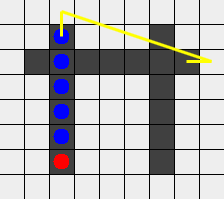
\includegraphics[width=.75\linewidth]{pics/transitionBefore.png}\\
        \captionof{figure}[vorZug]{Karte vor dem Zug}
        \label{fig:vorZug}
    \end{minipage}
    \hfill
    \begin{minipage}[t]{0.45\linewidth}
        \centering
        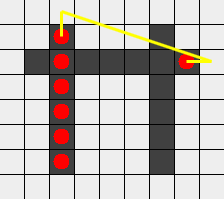
\includegraphics[width=.75\linewidth]{pics/transitionAfter.png}\\
        \captionof{figure}[nachZug]{Karte nach dem Zug}
        \label{fig:nachZug}
    \end{minipage}
\\

Zusätzlich wird die erweiterte Variante auf verschieden geformten Karten mit bis zu 8 Spielern gleichzeitig gespielt, wie in Abbildung \ref{fig:vorBombe}.\\ 
Hinzu kommt, dass ReversiXT aus zwei Phasen besteht, der herkömmlichen Spielphase und einer Bombenphase die eintritt, wenn keiner der Spieler einen möglichen Zug mehr hat. In dieser können die Spieler Bomben mit einer von der Karte vorgeschriebenen Stärke werfen um die feindlichen Steine zu dezimieren und die Menge ihrer eigenen Steine zu optimieren. Am Ende sieht das Spielfeld aus wie in Abbildung \ref{fig:nachBombe}. \\

	\begin{minipage}[t]{0.45\linewidth}
        \centering
        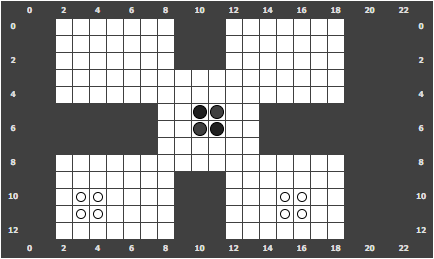
\includegraphics[width=1\linewidth]{pics/gamefield03.png}\\
        \captionof{figure}[vorBombe]{13x23-Karte zu Beginn des Spiels}
        \label{fig:vorBombe}
    \end{minipage}
    \hfill
    \begin{minipage}[t]{0.45\linewidth}
        \centering
        \includegraphics[width=1\linewidth]{pics/gamefield03afterbombphase.png}\\
        \captionof{figure}[nachBombe]{13x23-Karte nach Bombenphase}
        \label{fig:nachBombe}
    \end{minipage}
\\

Da dieses Wahlpflichtfach unser erstes vollständiges Projekt ist, verspricht man sich hiervon ein besseres logisches Verständnis von K.I.s, Algorithmen und eine Verbesserung der persönlichen Programmierfähigkeiten. Außerdem wird die Arbeit in der Gruppe gut für die Förderung der Teamfähigkeit sein.


\newpage
% ----------------------------------------------------------------------------------
% Kapitel: Allgemeine Informationen
% ----------------------------------------------------------------------------------
\section{Allgemeine Informationen}
Im Folgenden wird etwas genauer auf die Mitglieder des Teams, die Arbeitseinteilung und Kommunikationswege eingegangen.
Außerdem werden technische Daten und der Aufbau der Datenstruktur des Programmes genauer beschrieben.
\subsection{Team und Kommunikation}
Das Team setzt sich aus Burhan Köseler (3.Semester/Allgemeine Informatik), Vinzent Penzkofer (3.Semester/Allgemeine Informatik) und Christoph Bohren (4.Semester/Allgemeine Informatik) zusammen.
Die Vorbildung der Teammitglieder ist identisch, da alle Mitglieder im zweiten Semester Java behandelt haben.
Zum Austausch von Informationen und Code werden vor allem das Git-Gruppen-Repository, Discord\label{Discord} sowie WhatsApp\label{WhatsApp} benutzt.
Da die Aufgaben oft zu umfangreich sind um in der Veranstaltung am Montag bearbeitet zu werden treffen wir uns meistens Donnerstags oder spontan an der OTH Regensburg um gemeinsam am Projekt weiter zu arbeiten.\\
In der folgenden Tabelle \ref{tab:Aufgaben} wird die Aufgabenverteilung der einzelnen Gruppenmitglieder in den einzelnen Wochen dargestellt.

\begin{table}[]
\centering
\begin{tabular}{|c|c|c|c|}
\hline
*        & \begin{tabular}[c]{@{}c@{}}Vinzent\\ Penzkofer\end{tabular} & \begin{tabular}[c]{@{}c@{}}Burhan\\ Köseler\end{tabular} & \begin{tabular}[c]{@{}c@{}}Christoph\\ Bohren\end{tabular} \\ \hline
Woche 1  & Aufgabe 1.3+1.5 & Aufgabe 1.3+1.5 & Aufgabe 1.3+1.5 \\ \hline
Woche 2  & Aufgabe 2.2 & Aufgabe 2.1+2.3 & Aufgabe 3.2 \\ \hline
Woche 3  & Projektbericht & Aufgabe 3.1+Projektbericht & Aufgabe 3.2\\ \hline
Woche 4  & Aufgabe 3.1 & Aufgabe 2.1+2.3 & Aufgabe 3.2 \\ \hline
Woche 5  & Aufgabe 4.1+4.2 & Aufgabe 2.1+2.3 & Aufgabe 3.2 \\ \hline
Woche 6  & Aufgabe 4.1+4.2 & Aufgabe 2.1+2.3 & Aufgabe 3.2\\ \hline
Woche 7  & Aufgabe 5+6.2 & Aufgabe 5 & Aufgabe 3.2 \\ \hline
Woche 8  & Aufgabe 6.1 & Aufgabe 6.3+6.4+7 & Projektbericht \\ \hline
Woche 9  & Aufgabe 8.1 & Aufgabe 8.2 & Projektbericht \\ \hline
Woche 10 & Aufgabe 9.3 & Aufgabe 9.2 & Projektbericht \\ \hline
Woche 11 & Aufgabe 10 & Projektbericht & Projektbericht \\ \hline
Woche 12 & Aufgabe 10 + Projektbericht & Aufgabe 11 + Projektbericht &13.1 + Projektbericht\\ \hline
\end{tabular}
\caption{Aufgabenverteilung}
\label{tab:Aufgaben}
\end{table}


\subsection{Technische Daten}
Für die Implementierung des Projektes haben wird uns für die Programmiersprache Java (Java 12) entschieden.
Programmiert werden unter Windows 10\label{Windows 10} und Ubuntu Linux\label{Ubuntu} mithilfe der IDE IntelliJ (Version: 2019.1)\label{IntelliJ}.
Außerdem werden von Zeit zu Zeit Editoren wie z.B. Atom\label{Atom} und Notepad++\label{Notepad} hinzugezogen um  einen besseren Überblick über die vorhandenen Klassen zu gewinnen.
Die Entscheidung die K.I. in Java zu entwickeln fiel uns relativ leicht, da alle 3 Mitglieder der Gruppe mehr Erfahrung mit dieser Programmiersprache besitzen und sich die Implementierung von ausgearbeiteten Funktionalitäten und Algorithmen somit leichter gestaltet.
Ausgeführt und getestet wurde ob das Programm ob die Karten richtig einliest, gültige Spielzüge findet und ausführt sowohl und gesamte Spiele von Anfang bis Ende durchspielt auf den von der OTH gegebenen Rechnern als auch mit einem Rechner mit einem i7-6700k @3,6Ghz und 16GB DDR3 RAM. Desweiteren, wurden Laptops von Dell und Microsoft genutzt.

\subsection{Datenstruktur}
Unsere Datenstruktur besteht aus einer Klasse \texttt{Spielfeld}, welche die vom Server überlieferte Karte und die darin enthaltende Information abspeichert. \\
Spielerzahl, Anzahl der Überschreibsteine, Bomben, Bombenstärke sowie die Spielfeldhöhe bzw. Spielfeldbreite werden als Integer abgespeichert. \\
Das Spielfeld an sich und die hierin inbegriffenen einzelnen Felder werden in einem 2-Dimensionalen Char Array abgespeichert, wobei eine Dimension die Zeilen und die andere die Spalten des Spielfeldes beschreibt. \\
Die Transitionen werden in Form einer Liste von Integer Arrays gesichert. Diese beinhaltet die einzelnen Transitionen und damit jeweils deren Ein- bzw. Ausgangsorte und die jeweiligen Richtungen. \\
Außerdem gibt es die Klasse \texttt{GameState} welche für die Funktionen der K.I. wie das Abfragen von gültigen Zügen und ausführen eines Zuges dient. \\
Desweiteren, gibt es die Klassen \texttt{Client} und \texttt{HelperClassNetwork}, welche mit dem Server kommunizieren und die übertragenen Informationen verarbeiten und ausführen.\\ 
In \texttt{KIAlgorithmus} wurden Minimax mit \emph{Paranoid-Suche} und \emph{$\alpha$-$\beta$-Pruning} implementiert. \\
Ihre Effizienz wird in \texttt{Statistics} durch das Durchführen von Messungen (Vgl. Kapitel 4) bewertet. \\
In der Klasse \texttt{GameInfo} werden die gesetzten Flags beim Starten des Clients gespeichert. \\
Die Klasse \texttt{Node} wird dafür genutzt um bestimmte Daten, wie die nächsten Knoten eines Binärbaums zu speichern.   \\
\texttt{Player} dient als Container für die Werte des eigenen Spielers (z.B.: Bombenanzahl) und die benötigten Daten der gegnerischen Spieler. \\
Die von der Webseite Fightclub benötigte Schnittstelle zum Testen wird von \texttt{JSONFormatter} verwaltet. \\
Mit der Klasse \texttt{ComplexRating} bewerten wir die Knoten in der tiefsten Ebene um den best möglichen Spielzug auszuwählen. \\
Weiterhin gibt es die Klasse \texttt{RatingValues}, welche Werte enthaltet für die einzelnen Kriterien um einzelne Spielsituationen zu bewerten, z.B. wie wichtig es für die Heuristik ist eine Ecke einzunehmen oder Bonusfelder zu erreichen. \\
Die Klasse \texttt{SimpleRating} bewertet Spielzüge mit einer einfachen Logik und ermöglicht es die bestimmten Knoten im Baum zu sortieren um mit Hilfe des \emph{$\alpha$-$\beta$-Pruning} frühzeitig einen Ast des Binärbaums, welcher bei der \emph{Paranoid-Suche} entsteht, \glqq abzuschneiden\grqq und die Suche zu verkürzen. \\
Um die Statistiken der Klasse \texttt{Statistics} auswerten zu können, wird die Klasse  \texttt{RevXTLogger} genutzt. Diese schreibt die benötigten Werte aus den Statistiken heraus in eine .csv-Datei, welche man direkt in eine Excel-Tabelle einlesen kann.\\
Zuletzt gibt es die Klasse \texttt{Evaluator}, welche sich um die Bewertung der einzelnen Spielfeldsituation kümmern soll.

%Beschreiben Sie detailliert die Datenstruktur, die Sie zur Speicherung des Spielfeldes in Ihrem GameState nutzen. Gehen Sie auf Besonderheiten ein und erklären Sie, wie diese funktionieren und was Sie sich davon erhoffen. Gehen Sie auf die Vorteile (und evtl.\ Nachteile) ein, die Ihre Datenstruktur aus Ihrer Sicht hat. Geben Sie falls möglich auch eine schematische Darstellung/ein Bild der Datenstruktur an. Klären Sie insbesondere auch, wie Transitionen bei Ihnen repräsentiert werden. Auch hier könnte ein schematisches Bild beim Verständnis helfen.

%Der Umfang dieses Abschnitts sollte mindestens eine $\frac{3}{4}$-Seite betragen.


\newpage
% ----------------------------------------------------------------------------------
% Kapitel: Spielfeldbewertung
% ----------------------------------------------------------------------------------
\section{Spielfeldbewertung}
Im Folgenden Kapitel wird die Bewertung der jeweiligen Spielfeldsituationen und die Implementierung der Heuristiken sowie deren Kriterien und Funktionsweise behandelt.

\subsection{Kurzübersicht}
Unsere Heuristik besteht aus zwei Instanzen, die zwar unabhängig operieren sich aber gleichzeitig gegenseitig zuarbeiten. Hier soll kurz erklärt werden wie diese Zusammenarbeit funktioniert. \\
Das Ziel der ersten Instanz, der Tiefenheuristik, ist es die Vorteile des Paranoid-Algorithmus voll auszunutzen. Dabei werden in möglichst großer Tiefe die Spielstände simuliert und ausgewertet. Diese Auswertung ist sehr simpel, da diese Bewertung eines Spielstands nur einige wenige Kriterien miteinbezieht, um den Einfluss der verschiedenen Faktoren möglichst übersichtlich und leicht nachvollziehbar zu halten. Die einzelnen Faktoren werden später noch genauer beschrieben.\\
Die zweite Instanz, die sogenannten Kurzschlussentscheidungen, arbeiten extrem effizient. Kurzschlussentscheidungen sind immer Spielzüge, die eine starke Verbesserung der Spielsituation herbeiführen, allerdings nur relativ selten im Verlauf eines Spiels auftreten. Ein Beispiel hierfür (die anderen werden später noch genauer erläutert), wäre das Erobern eines Bonusfeldes. Diese Chancen, die die Spielsituation des Clients erheblich zu verbessern, müssen auf jeden Fall genutzt werden. Deshalb wird in Tiefe 1 eine Kurzschlussentscheidung gefällt und ohne weitere Betrachtung des Baumes, dieser sehr günstige Zug ausgeführt.\\
Die Hautaufgabe der Tiefenheuristik ist folglich, solche Chancen mit erhöhter Wahrscheinlichkeit herbeizuführen. Diese können schließlich, mit Hilfe von Kurzschlussentscheidungen, sehr schnell identifiziert und ausgenutzt werden.\\


\subsection{Tiefenheuristik}
  
Die Tiefenheuristik setzt sich aus 3 Hauptkomponenten zusammen. Diese werden im Folgenden einzeln behandelt und erklärt:\\
 
 \begin{itemize}
 \item Statische Heuristik\\
 Diese Heuristik wertet ein gegebenes Spielfeld aus und entscheidet welche 	 Felder günstig, neutral oder ungünstig sind. Dabei weist sie jedem   besetzbarem Feld einen Wert zwischen -10 (sehr schlecht) und 10 (sehr gut) zu. Die Güte eines Feldes wird nach folgenden Faktoren bestimmt.
Feld ist:

 
 
 	\begin{itemize}
 		\item{Kante: Güte += 1}
 		\item{Eckfeld: Güte += 3}
 		\item{Feld mit Abstand 1 zu einem Eckfeld: Güte -= 2}
 		\item{Bonusfeld: Güte += 7}
 		\item{Feld mit Abstand 2 zu einem Bonusfeld: Güte += 4}
 		\item{Feld mit Abstand 1 zu einem Bonusfeld: Güte -= 3}
 	\end{itemize}
 		
 \item{Dynamische Bewertung}
 In die dynamische Bewertung fließen alle Faktoren ein, die sich im Verlauf des Spiels ändern. Diese Faktoren werden jedes mal neu berechnet.\\
 Kriterien:
  \begin{itemize}
  \item{Anzahl der Steine die Momentan im eigenen Besitz sind}
  \item Mobilität, bzw. die Anzahl der möglichen Züge
  \item Hierarchie, bzw. die momentane Platzierung im Vergleich zu den anderen Spielern
  
  \end{itemize}
  \item Bonusfeldbewertung:\\
  Da die Überschreibsteine eine ganz entscheidende Rolle beim Ausgang eines Matches spielen, haben diese nochmal eine eigene Bewertung. Der Vorteil dabei ist, dass die Bonusfelder nochmal unabhängig von der statischen Bewertung gewichtet werden können. Die Bonusfeldheuristik soll möglichst viele Situationen erzeugen, bei denen ein Bonusfeld eingenommen werden kann.\\
  Kriterien:
  \begin{itemize}
  \item Bonusfeld eingenommen
  \item Feld mit Abstand 2 zu einem Bonusfeld eingenommen
  \item Feld mit Abstand 1 zu einem Bonusfeld eingenommen
  \begin{itemize}
  \item Schlecht da es einem anderen Spieler ermöglicht wird das Bonusfeld einzunehmen
  \end{itemize}
  \item \textit{Ausblick: Abstand zum nächsten Bonusfeld miteinbeziehen}
  \end{itemize}
 \end{itemize}
 
Für alle drei Hauptkomponenten wird ein prozentualer Wert berechnet, welcher beschreibt inwiefern sich der tatsächliche aktuelle Spielstand im Vergleich zu dem zu bewertenden Spielstand verbessern/verschlechtern würde.

\begin{equation}
 Verbesserung = \frac{ZuBewertenderSpielstand}{AktuellerSpielstand} \nonumber
\end{equation}

Dabei gilt:
\begin{align}
	Verbesserung > 1 &: Spielstand\, hat\, sich\, verbessert \nonumber \\ 
	Verbesserung = 1 &: Spielsituation\, ist\, gleich \nonumber \\
	Verbesserung < 1 &: Spielsituation\, hat\, sich\, verschlechtert \nonumber
\end{align}  

\textbf{Beispiel:}
Der Client besitzt bereits 20 Steine und bewertet nun in Tiefe d einen Spielstand, in dem er 25 Steine besitzt, bei gleichbleibend vielen möglichen Zügen und gleicher Platzierung im Vergleich zur aktuellen Situation. 

\begin{align}
	Verbesserung_{dynamisch} &= \frac{ZuBewertenderSpielstand}{AktuellerSpielstand} \nonumber \\
	Verbesserung_{dynamisch} &= \frac{25}{20} \nonumber \\
	Verbesserung_{dynamisch} &= 1.25 \nonumber
\end{align}

Die Spielsituation hat sich im Bereich Dynamik folglich um 25\% verbessert.\\
Dieser Wert für die Verbesserung $V(Bereich)$ wird jeweils mit 100 und einem Gewichtungsfaktor $g_{Bereich}$ multipliziert, um die Gesamtbewertung des Spielstands zu berechnen.
\begin{align}
Bewertung = 100*g_{dynamisch}*V(dynamisch)+100*g_{statisch}*V(statisch)+100*g_{bonus}*V(bonus)\nonumber
\end{align}

Dies ist die abschließende Bewertung des Spielstandes, die für alle untersten Knoten des Spielbaums berechnet und anschließend an den Paranoid-Algorithmus zurückgegeben wird. Dabei sind die konkreten Werte für Gewichtungsfaktoren und die Wertigkeit eines bestimmten Feldes jederzeit anpassbar, um eine Feineinstellung zu ermöglichen.   

\subsection{Kurzschlussheuristik}
Der zweite wesentliche Teil unserer Heuristik erntet die Früchte der Tiefenheuristik. Hier werden die Chancen, die wir mit der Tiefenheuristik versuchen herbeizuführen, ergriffen. Dabei wird in Tiefe 1, also in den unmittelbar folgenden Spielständen, nach Möglichkeiten gesucht, die einen großen positiven Einfluss auf die eigene Spielsituation haben. Diese Situationen müssen folgende Bedingungen erfüllen.

\begin{itemize}
\item D"urfen nicht zu oft auftreten
\item M"ussen die Spielsituation erheblich verbessern
\end{itemize}

Das ist wichtig, denn für eine Kurzschlussentscheidung wird die Tiefensuche komplett übersprungen. Jedoch darf dies nicht zu oft passieren, da man sonst den Vorteil des \glqq Blicks in die Zukunft\grqq{}, den der Paranoid-Algorithmus bietet, verliert und muss die Spielsituation so signifikant verbessern, dass es sehr unwahrscheinlich ist, durch die Tiefensuche einen besseren Zug zu finden.\\
Falls eine solche Situation gefunden wird, kann der Spielzug sofort gemacht werden.

Hierbei sind die Vorteile:

\begin{itemize}
\item Deutliche Zeitersparnis (nur die Folgespielstände in Tiefe 1 müssen durchsucht werden)
\item Kein Risiko einer Fehlentscheidung\\
	$\Rightarrow$ In der Tiefe spielen viele Faktoren eine Rolle, die nur schwer einzuschätzen sind und es gibt keine Garantie, dass ein günstiger Zustand tatsächlich eintritt 
\end{itemize}

Folgende Spielsituationen lösen eine Kurzschlussentscheidung aus:
	\begin{itemize}
	\item Erobern eines Bonusfeldes
	\item Erobern eines Eckfeldes (wird deaktiviert falls zu viele Eckfelder auf einer Karte)
	\item Erobern eines Feldes mit Abstand 2 zum nächsten Bonusfeld
	\end{itemize}
	
Theoretisch könnten noch weitere Fälle, wenn sie die oben genannten Bedingungen erfüllen, hinzugefügt werden. Dabei sollte man aber immer im Blick behalten, dass alle Kurzschlussentscheidungen kombiniert nur einen kleinen Anteil an allen gemachten Zügen haben sollten. Ansonsten wird der Nutzen des Paranoid-Algorithmus eingeschränkt.

\subsection{Override Mode}
Da der sinnvolle Einsatz von Überschreibsteinen in sehr vielen Matches spielentscheidend ist, wurde dieser Fall in der Heuristik gesondert betrachtet. Überschreibsteine werden (Ausnahmefälle werden vernachlässigt) am besten am Ende des Spieles benutzt, da dort der Effekt am größten ausfällt. Unter dieser Annahme ist es nicht sinnvoll, die Überschreibsteine während des restlichen Spiels miteinzubeziehen, da sie zum einen nicht benutzt werden sollten und zum andern den Suchbaum extrem ausweiten (jedes besetzte Spielfeld ist ein potentieller Zug). Deshalb werden bei der Suche nach möglichen Zügen, die Überschreibsteine nur dann miteinbezogen wenn die Suche ansonsten keinen Zug findet.\\
Wenn der Fall schließlich doch einmal eintritt, geht die Heuristik in den Override Mode über. Das bedeutet, dass versucht wird, entweder die Mobilität $(Spielfortschritt < 90\%)$, oder die Gesamtzahl der Steine zu maximieren $(Spielfortschritt >= 90\%)$. Alle anderen Einflussfaktoren werden anschließend vernachlässigt.

	
	

\newpage
% ----------------------------------------------------------------------------------
% Kapitel: Statistiken
% ----------------------------------------------------------------------------------
\section{Statistiken}
%Versuchen Sie erneut eine \emph{weiche} Überleitung in dieses Kapitel zu formulieren, indem Sie kurz beschreiben, was den Leser in diesem Kapitel erwartet und warum das für die Thematik interessant ist.
Neben Heuristiken ist die Effizienz der verwendeten Algorithmen maßgeblich verantwortlich dafür wie gut der Client spielen kann. So soll er sowohl eine möglichst große Zahl von Zügen vorausberechnen können (Tiefe im Baum), als auch möglichst wenig Rechenzeit dafür benötigen. Im Folgenden wird die Effizienz des Paranoid-Algorithmus inklusive \emph{Paranoid-Suche} mit der des um \emph{$\alpha$-$\beta$-Pruning} erweiterten Algorithmus, in mehreren Messungen, mit jeweils verschiedener Tiefe im Baum, verglichen.


\subsection{Vergleich von Paranoid-Suche mit $\boldsymbol{\alpha}$-$\boldsymbol{\beta}$-Pruning}

Zunächst soll kurz das Vorgehen bei der Erstellung der Daten erläutert werden. \\
Damit die Daten möglichst automatisiert erstellt werden konnten, wurden \texttt{bash-}Skripte zur mehrfachen Ausführung von Spielen geschrieben. Ein Skript diente zum Verbindungsaufbau mit dem Server über den die Spiele liefen, zwei bzw. drei Weitere führten die Clients aus und ein Letztes rief alle anderen Skripte parallel auf. Zusätzlich wurde der Client um die Logger-Klasse \texttt{RevXTLogger} erweitert, die Daten, wie die expandierten Zustände je Zug oder die für einen Zug benötigte Zeit in Millisekunden, in eine \texttt{CSV-}Datei logt. Log-Dateien wurden dann jeweils von zwei am Spiel beteiligten Clients erstellt und ausgewertet.\\
Anschließend wurde für jedes durchgeführte Spiel, per Excel, das arithmetische Mittel aus den je Zug expandierten Zuständen und der dafür benötigten Zeit in Millisekunden berechnet. Die so gewonnenen Werte wurden dann selektiert nach Tiefe und Karte in eine weitere Excel-Datei zusammengetragen. Dann wurde abermals das arithmetische Mittel gebildet, um die Mittelwerte für jede Karte zu ermitteln. Danach konnten sie in den unten aufgeführten tabellarischen Gesamtvergleich eingetragen werden.\\
Interessant ist es aber auch die Zahl der expandierten Zustände in Abhängigkeit von der Suchtiefe zu beobachten. Dazu wurde aus den im Gesamtvergleich abgebildeten arithmetischen Mitteln nochmals, sortiert nach den jeweiligen Tiefen, das arithmetische Mittel gebildet, sodass nun für jede Suchtiefe ein Mittelwert existierte, der alle vier verwendeten Karten berücksichtigt.\\
  
\vspace{1em}
\begin{minipage}{\linewidth}
	\centering
	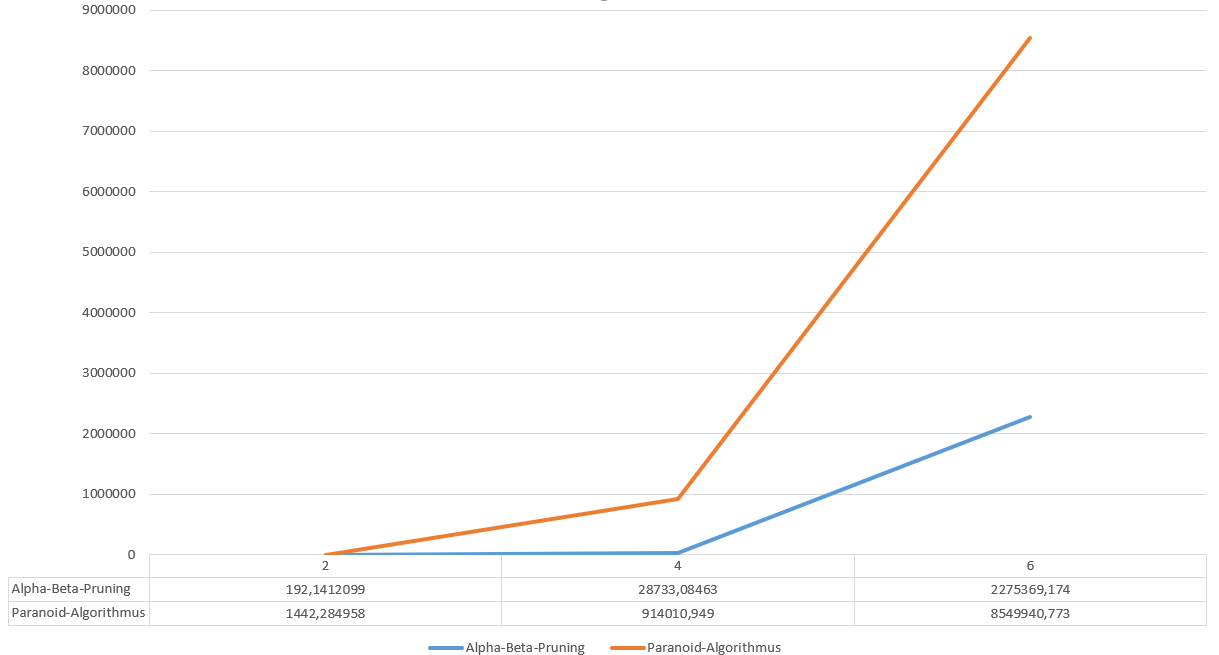
\includegraphics[width=0.9\linewidth]{pics/VglABParanoid.png}
	\captionof{figure}[VglAlphaBetaParanoid]{Vergleich Alpha-Beta-Pruning und Paranoid-Suche}
	\label{fig:VglAlphaBetaBaranoid}
\end{minipage}

Hinsichtlich der Zahl expandierter Zustände im Verhältnis zur Suchtiefe, lassen sich zwischen \emph{Paranoid-Suche} und einem um $\alpha$-$\beta$-Pruning erweiterten Algorithmus erhebliche Unterschiede feststellen. 
Diese sind umso größer, je höher die Suchtiefe ist. So beträgt die durchschnittliche Zahl expandierter Zustände bei Tiefe sechs 8549940,77, wenn kein $\alpha$-$\beta$-Pruning verwendet wird und 2275369,17 wenn es genutzt wird. 
Es ergibt sich hieraus also eine Differenz von über sechs-Millionen Zuständen und eine enorme Performance-Verbesserung und Zeitersparnis. 
Das resultiert daraus, dass durch das Wegschneiden uninteressanter Äste beim $\alpha$-$\beta$-Pruning, der Verzweigungsgrad des Suchbaums halbiert wird.
Bei Tiefe zwei fällt dieser Gewinn, aufgrund der kleineren Gesamtzahl an Zuständen erheblich geringer aus. 1442,28 Zustände müssen ohne die Hinzunahme von $\alpha$-$\beta$-Pruning untersucht werden und 192,14 mit. Es ist hier allerdings anzumerken, dass der Gewinn hinsichtlich des halbierten Verzweigungsgrades gleich bleibt.\\

Im Folgenden werden nun die zur Erstellung der Statistiken verwendeten Karten und ein tabellarischer Gesamtvergleich der Verfahren $\alpha$-$\beta$-Pruning einerseits und reiner \emph{Paranoid-Suche} andererseits vorgestellt. Die Karten sind unterschiedlich groß und verfügen dadurch, sowie wegen ihrer Zahl an Transitionen, über eine sehr unterschiedliche Zahl von Zugmöglichkeiten. Aufgrund des sehr hohen Zeitaufwands, den die Spiele auf höheren Suchtiefen benötigten, wurden nicht überall gleich viele Spiele durchgeführt. Gemessen wurden die durchschnittliche Zahl an expandierten Zuständen pro Spielzug (gekennzeichnet mit "n") und die dafür benötigte Zeit in Millisekunden.\\

\vspace{1em}

\textbf{Legende:}\\[1em]
\begin{tabular}{cccc}
  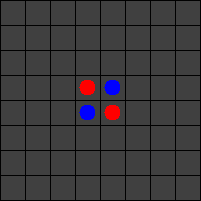
\includegraphics[width=0.22\linewidth]{maps/reversi-orig_2p.png}&
  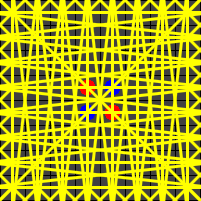
\includegraphics[width=0.22\linewidth]{maps/reversi-transitionen_2p.png}&
  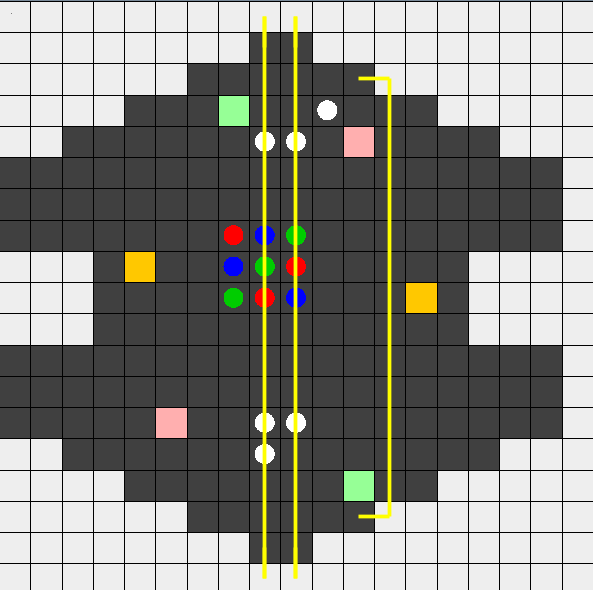
\includegraphics[width=0.22\linewidth]{maps/pfeil_3p.png}&
  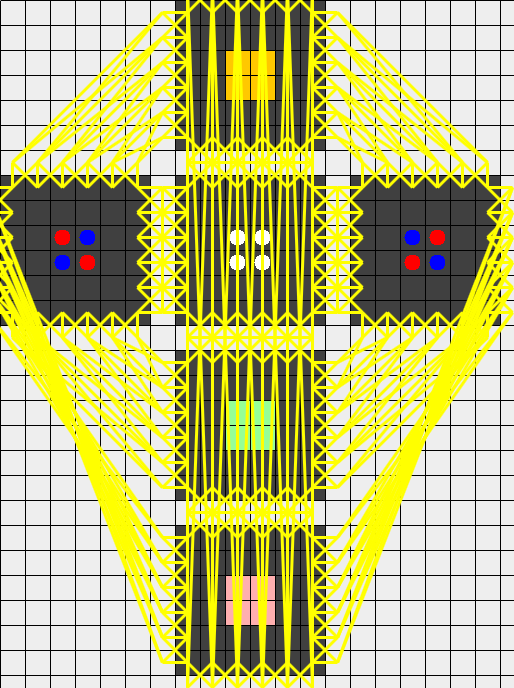
\includegraphics[width=0.22\linewidth]{maps/wuerfel_2p.png}
  \\
  \scriptsize 1.~\texttt{reversi-orig\_2p.map}&
  \scriptsize 2.~\texttt{reversi-transitionen\_2p.map}&
  \scriptsize 3.~\texttt{pfeil\_3p.map}&
  \scriptsize 4.~\texttt{wuerfel\_2p.map}
\end{tabular}


\subsection{Gesamtvergleich (Tiefe = 2)}
\newcolumntype{L}[1]{>{\raggedright\let\newline\\\arraybackslash\hspace{0pt}}m{#1}}
\newcolumntype{C}[1]{>{\centering\let\newline\\\arraybackslash\hspace{0pt}}m{#1}}
\newcolumntype{R}[1]{>{\raggedleft\let\newline\\\arraybackslash\hspace{0pt}}m{#1}}
\begin{tabular}{|c|L{1.5cm}|R{6.5cm}|R{6.5cm}|}
\hline
\centering\textbf{Karte}&
\centering\textbf{Anzahl Spiele}&
\centering\textbf{Paranoid-Suche}&
$\boldsymbol{\alpha}$-$\boldsymbol{\beta}$-Pruning\\\hline\hline
1.&25&80.77 n; 6.49 ms&41.53 n; 4.05 ms\\\hline
2.&25&562.86 n; 35.58 ms &86.34 n; 11.41 ms\\\hline
3.&25&3902.14 n; 162 ms&376.61 n; 40.04 ms\\\hline
4.&25&1223.37 n; 231.42 ms&264.08 n;  98.45 ms\\\hline
\end{tabular}\\

\subsection{Gesamtvergleich (Tiefe = 4)}
\newcolumntype{L}[1]{>{\raggedright\let\newline\\\arraybackslash\hspace{0pt}}m{#1}}
\newcolumntype{C}[1]{>{\centering\let\newline\\\arraybackslash\hspace{0pt}}m{#1}}
\newcolumntype{R}[1]{>{\raggedleft\let\newline\\\arraybackslash\hspace{0pt}}m{#1}}
\begin{tabular}{|c|L{1.5cm}|R{6.5cm}|R{6.5cm}|}
\hline
\centering\textbf{Karte}&
\centering\textbf{Anzahl Spiele}&
\centering\textbf{Paranoid-Suche}&
$\boldsymbol{\alpha}$-$\boldsymbol{\beta}$-Pruning\\\hline\hline
1.&25&7630,91 n; 198,99 ms&735,96 n; 28,43 ms\\\hline
2.&24&1960752,23 n; 30490,44 ms&4682,36 n; 174,68 ms\\\hline
3.&10&293239,09 n; 15695,2 ms&64252,69 n; 3483,68 ms\\\hline
4.&5&1394421,58 n; 266532,4275 ms&45261,33 n; 7846,13 ms\\\hline
\end{tabular}\\

\subsection{Gesamtvergleich (Tiefe = 6)}
\newcolumntype{L}[1]{>{\raggedright\let\newline\\\arraybackslash\hspace{0pt}}m{#1}}
\newcolumntype{C}[1]{>{\centering\let\newline\\\arraybackslash\hspace{0pt}}m{#1}}
\newcolumntype{R}[1]{>{\raggedleft\let\newline\\\arraybackslash\hspace{0pt}}m{#1}}
\begin{tabular}{|c|L{1.5cm}|R{6.5cm}|R{6.5cm}|}
\hline
\centering\textbf{Karte}&
\centering\textbf{Anzahl Spiele}&
\centering\textbf{Paranoid-Suche}&
$\boldsymbol{\alpha}$-$\boldsymbol{\beta}$-Pruning\\\hline\hline
	1.&25&1110986,42 n; 12786,13 ms&26478,52 n; 217,15 ms\\\hline
	2.&5&8763449,79 n; 153303,22 ms&181053,04 n; 2521,06 ms\\\hline
	3.&1&18582166,32 n; 580842,81 ms&4528852,73 n; 164786,73 ms\\\hline
	4.&1&5743160,56 n; 1694718,12 ms&4365092,4 n; 1619458,65 ms\\\hline
\end{tabular}\\

Beim tabellarischen Vergleich der Verfahren $\alpha$-$\beta$-Pruning und \emph{Paranoid-Suche} fallen ähnliche Unterschiede auf, wie bereits in Abbildung \ref{fig:VglAlphaBetaBaranoid} dargestellt. \\
Mit der Zunahme der Suchtiefe werden auf den gleichen Karten deutlich mehr Zustände expandiert. So werden auf Karte eins mit einer Tiefe von zwei etwa 80,77, auf Tiefe vier bereits 7630, 91 und auf Tiefe sechs 1110986,42 Zustände expandiert. Es lässt sich also durchaus von exponentiellem Wachstum sprechen. \\
Zudem fällt der enorme Gewinn auf, der durch die Verwendung von $\alpha$-$\beta$-Pruning erzielt wird. Das fällt mehr auf, je höher der Verzweigungsgrad im Spielbaum ist. Der Client expandiert etwa auf Karte zwei, bei Tiefe vier 1960752,23 Zustände, wenn nur \emph{Paranoid-Suche} verwendet wird. Wird er dagegen mit $\alpha$-$\beta$-Pruning ergänzt, werden nur 4682,36 Zustände untersucht und der Zug dauert 174,68 ms statt 30490 ms.\\
Auf der gleichen Karte expandiert der Client, auf Tiefe sechs, lediglich 181053,04 statt 8763449,79 Zustände und benötigt dafür durchschnittlich 2521 ms im Vergleich zu 153303,22 ms.\\
Der Client kann also durch die beträchtliche Zeitersparnis bessere Züge machen, wenn  $\alpha$-$\beta$-Pruning eingesetzt wird.
Weiterhin lässt sich aufzeigen, dass die Zahl expandierter Zustände auf unterschiedlichen Karten bei derselben Tiefe höchst unterschiedlich sein kann. So wurden auf Karte fünf bei einer Suchtiefe von vier im Schnitt 1394421,58 auf Karte zwei 1960752,23 und auf Karte eins nur 7630,91 Zustände untersucht. Das lässt sich, gerade wenn man Karte eins und Karte zwei miteinander vergleicht, durch eine weit höhere Zahl von Zugmöglichkeiten, bedingt etwa durch Transitionen, erklären. 

\newpage

\subsection{Gesamtvergleich (Zeit = 2 Sekunden)}
\newcolumntype{L}[1]{>{\raggedright\let\newline\\\arraybackslash\hspace{0pt}}m{#1}}
\newcolumntype{C}[1]{>{\centering\let\newline\\\arraybackslash\hspace{0pt}}m{#1}}
\newcolumntype{R}[1]{>{\raggedleft\let\newline\\\arraybackslash\hspace{0pt}}m{#1}}
\begin{tabular}{|c|L{1.5cm}|R{6.5cm}|R{6.5cm}|}
\hline
\centering\textbf{Karte}&
\centering\textbf{Anzahl Spiele} &
\centering\textbf{Paranoid-Suche}&
$\boldsymbol{\alpha}$-$\boldsymbol{\beta}$-Pruning\\\hline\hline
1.&10&86319,29 n&73642,62 n\\\hline
2.&10&44264,71 n&31947,93 n\\\hline
3.&10&26442,19 n&23039,41 n\\\hline
4.&10&15527,92 n&11545,09 n\\\hline
\end{tabular}\\

Der Unterschied in der Anzahl von expandierten Zuständen zwischen $\alpha$-$\beta$-Pruning und \emph{Paranoid-Suche} fällt beim Spiel auf Zeit sichtlich geringer aus, als beim Spiel auf Tiefe. Dennoch expandiert der Minimax-Algorithmus mit Paranoid-Suche meistens mehr Knoten, als derselbe mit $\alpha$-$\beta$-Pruning. So werden bei Karte eins 86319,29 Spielzustände per \emph{Paranoid-Suche} untersucht und 73642,62 mit $\alpha$-$\beta$-Pruning. Der relativ geringe Unterschied könnte auf das Zeitlimit zurückzuführen sein. Es bleibt möglicherweise nicht genug Zeit, um die Vorteile des  $\alpha$-$\beta$-Pruning vollumfänglich auszunutzen.\\
Auch fiel hinsichtlich der Zahl expandierter Zustände eine größere Unregelmäßigkeit auf, als bei einem Spiel auf Tiefe. Das ist vermutlich auch auf das Zeitlimit zurückzuführen. Bei einigen Zügen hat der Client mehr Zeit zur Berechnung und untersucht daher auch mehr Zustände.


\newpage
% ----------------------------------------------------------------------------------
% Kapitel: Eigene Spielfelder
% ----------------------------------------------------------------------------------
\section{Wettbewerbs-Spielfelder}
Nachdem bisher Algorithmen und Heuristiken des Clients beschrieben wurden, sollen nun die Spielfelder vorgestellt werden, die eigens für den Wettbewerb hinzugefügt wurden.
Die Heuristik des Clients bewertet Kanten, Ecken und Bonussteine höher als gewöhnliche Felder. Insbesondere die letzten Beiden wurden oft als spielentscheidend wahrgenommen und erzielen so hohe Bewertungen. Im Folgenden soll gezeigt werden, wie die eingereichten Spielfelder diese Strategie unterstützen.


\vspace{1em}
\begin{minipage}{\linewidth}
	\centering
	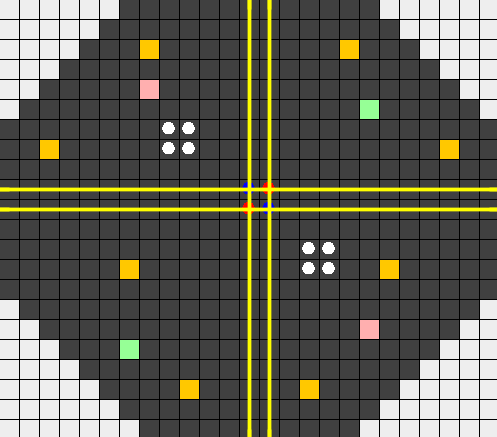
\includegraphics[width=0.6\linewidth]{pics/comp2019_04_2p.png}
	\captionof{figure}[compMap 01]{Wettbewerbsspielfeld für zwei Spieler}
	\label{fig:comp2p}
\end{minipage}
\vspace{1em}

In Abbildung \ref{fig:comp2p} ist deutlich eine achteckige Grundstruktur des Spielfelds zu erkennen. Außerdem finden sich hier eine, für die Größe des Spielfelds, hohe Zahl von Bonussteinen, die als Überschreibsteine genutzt werden können, auf dem Feld. Die anfängliche Zahl von Überschreibsteinen ist auf zwei Stück gesetzt, sodass die Spieler zu Beginn des Spiels nicht viele davon zur Verfügung haben. So ist es von großem Vorteil, wenn Bonussteine aufgesammelt werden. Da der vorliegende Client das besonders hoch gewichtet sollte hier leicht ein Vorteil errungen werden können. Transitionen finden nur an den Kanten statt, sodass durch sie keine Ecken verschwinden. Die Bombenzahl und -stärke wurde auf jeweils zwei festgesetzt, sodass sie nicht allzu stark ins Gewicht fallen sollten.  


\vspace{1em}
\begin{minipage}{\linewidth}
	\centering
	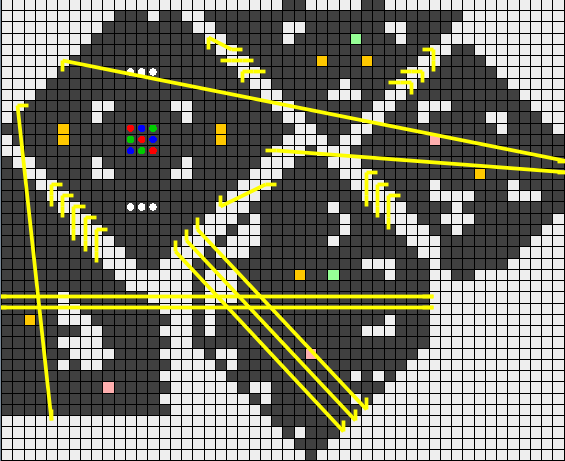
\includegraphics[width=0.6\linewidth]{pics/comp2019_04_3p.png}
	\captionof{figure}[compMap 02]{Wettbewerbsspielfeld für drei Spieler}
	\label{fig:comp3p}
\end{minipage}
\vspace{1em}



Wie aus Abbildung \ref{fig:comp3p} hervorgeht, wurde auch bei dem Spielfeld für drei Spieler auf eine relativ hohe Zahl von Ecken und Kanten geachtet, was für den Client generell von Vorteil sein dürfte. Das ist zum Teil auch dadurch erreicht worden, dass leere Felder in die einzelnen Spielbereiche eingefügt wurden.
Eine hohe Zahl von Bonussteinen stellt wie bei Abbildung \ref{fig:comp2p} sicher, dass der Client über sie in der späten ersten Spielphase einen Vorteil erreichen kann. Zu Spielbeginn starten alle Spieler mit keinerlei Überschreibsteinen und Bomben, sodass jeder Client enorm davon profitiert Bonussteine aufzusammeln. Es ist, wie zu Beginn des Kapitels erläutert, davon auszugehen, dass unser Client besonders viele Bonussteine aufsammeln wird.


\vspace{1em}
\begin{minipage}{\linewidth}
	\centering
	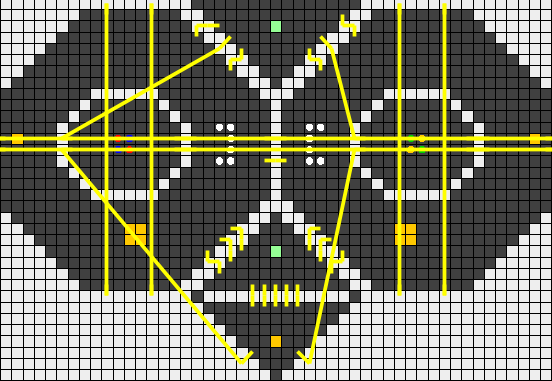
\includegraphics[width=0.6\linewidth]{pics/comp2019_04_4p.png}
	\captionof{figure}[compMap 03]{Wettbewerbsspielfeld für vier Spieler}
	\label{fig:comp4p}
\end{minipage}
\vspace{1em}

Die Spielkarte für vier Spieler, die für den Wettbewerb eingereicht wurde (siehe Abbildung \ref{fig:comp4p}) verfolgt dieselben Strategien wie die weiter oben beschriebenen Karten. Es wurde durch einige achteckige Strukturen auf eine relativ hohe Zahl von Ecken und Kanten geachtet, die vom Client gut ausgenutzt werden kann. Zu Spielbeginn verfügt kein Spieler über Bomben oder Überschreibsteine, sodass das Aufsammeln von Bonussteinen äußerst vorteilhaft ist.


\vspace{1em}
\begin{minipage}{\linewidth}
	\centering
	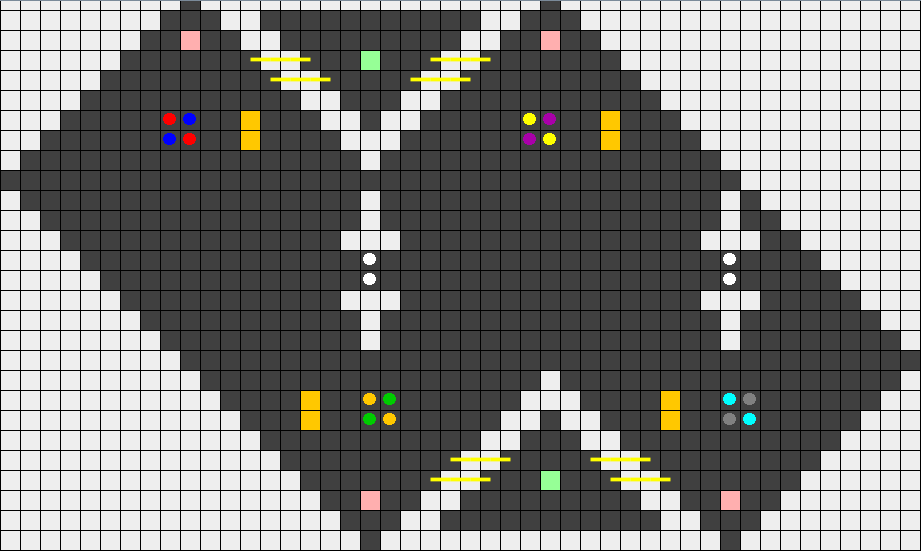
\includegraphics[width=0.6\linewidth]{pics/comp2019_04_8p.png}
	\captionof{figure}[compMap 04]{Wettbewerbsspielfeld für acht Spieler}
	\label{fig:comp8p}
\end{minipage}
\vspace{1em}

Abbildung \ref{fig:comp8p} stellt die Karte für acht Spieler dar und der Hauptspielbereich ist dem Teilgrundriss eines Ikosaeders nachempfunden, sodass eine ecken- und kantenreiche Grundstruktur entstanden ist. Mehr Ecken und Kanten wurden durch leere Felder in der Grundstruktur geschaffen, um dem Client weitere Gelegenheiten zu bieten sie zu besetzen. Jeder Spieler startet mit vier Bonussteinen und zwei Bomben mit jeweils Bombenstärke drei. In der Nähe jeder Startposition befinden sich zwei Bonussteine, wodurch der Client Gelegenheit erhält sich weitere Überschreibsteine zu sichern. Den sich daraus ergebenden Vorteil kann er dann vor der Bombenphase nutzen, um sich viele Spielsteine zu sichern. Bomben mit Bombenstärke drei sollten nicht zu viele davon zerstören können. 

\newpage
% ----------------------------------------------------------------------------------
% Kapitel: Fazit
% ----------------------------------------------------------------------------------
\section{Fazit}

Der Kurs erwies sich als stellenweise recht herausfordernd und es konnten einige neue Fähigkeiten erworben und verbessert werden. Dazu gehören zum Beispiel der Umgang mit LaTeX, die Verbesserung von Programmierkenntnissen, die Arbeit im Team, neue Algorithmen und die teils eigenständige Aneignung von diesen. Der Wettbewerb mit anderen Gruppen wurde als sehr anregend empfunden und die sichtbare Verbesserung des eigenen Clients motivierte sehr.
Problemsituationen kamen manchmal auf, wenn neue Fähigkeiten erworben werden mussten, konnten aber durch gegenseitige Hilfe im Team und eigene Arbeit gelöst werden.\\
Positiv fielen auch die zur Verfügung gestellten Werkzeuge, wie der Map-Editor oder der Fightclub auf. Vor allem Letzter vereinfachte die Verbesserung des eigenen Clients enorm.\\
Wünschenswert für den Fightclub wäre vor allen Dingen, dass sich Testspiele auch von Kursteilnehmern starten lassen.


\newpage


\pagebreak


% ----------------------------------------------------------------------------------------------------------
% Literatur
% ----------------------------------------------------------------------------------------------------------
\renewcommand\refname{Quellenverzeichnis}
\bibliographystyle{alpha}
\bibliography{quellen}
\section{Quellenverzeichnis}
https://im-zock:8091; letzter Zugriff: 12.05.2019, 13.13 Uhr\\
https://www.eclipse.org; letzter Zugriff: 12.07.2019, 20.03 Uhr\\
https://www.jetbrains.com/idea/; letzter Zugriff: 12.07.2019, 20.05 Uhr\\
https://notepad-plus-plus.org; letzter Zugriff: 12.07.2019, 20.07 Uhr\\
https://discordapp.com; letzter Zugriff: 12.07.2019, 20.34 Uhr\\
https://atom.io; letzter Zugriff: 12.07.2019, 20.05 Uhr\\
\pagebreak



\end{document}
